\chapter{Cryptanalysis of Simon}\label{ch:SIMON}
\section{Introduction}
Nowadays lightweight cryptography is rapidly evolving and becoming more and more important due to the increasing demand from mobile phones and Internet of Things. These lightweight cryptographic primitives are designed to
be efficient (in both hardware and software) when limited
hardware resources are available and at the same time to
guarantee a desired level of security. The
design of such primitives is a great challenge and can be
seen as a non-trivial optimization problem, where several
trade-offs are taken into account. They need to maintain
a reasonable balance between security, efficient software and hardware
implementation and very low overall cost with respect to several
meaningful metrics (power consumption, energy consumption,
size of the circuit \cite{OptimiPaper,BoyarPeraltaMCMethod,BoyarPeraltaMCBoolean}).

The research community has
proposed many lightweight hash functions, block ciphers and stream ciphers which are
reasonably good and satisfy at a reasonable level the trade-off
between efficiency and security. Nowadays, in the cryptographic
literature we find lots of such lightweight cryptographic primitives such as
KATAN \cite{KATAN}, KLEIN \cite{KLEIN}, ICEBERG
\cite{ICEBERG}, HIGHT \cite{HIGHT}, LED \cite{LED},
mCrypton \cite{mCrypton}, PRESENT \cite{PRESENT}, Piccolo \cite{Piccolo}
and many others.

In July 2013, a team from the NSA has proposed two new families of particularly lightweight block
ciphers, SIMON and SPECK, both coming in a variety of widths and key sizes
\cite{NSAciphers}. We use a basic reference implementation of both ciphers
which  can be found in \cite{simonref},
as well as the generator of algebraic equations to be used in algebraic attacks.

The designers published the full specifications and presented
only performance and implementation footprints, without providing
any advanced security analysis
against known cryptanalytic attacks.
Both of them offer excellent performance on both
hardware and software platforms and perform
exceptionally well across the majority of lightweight applications and
not only on a singe platform. Compared to
other lightweight cryptographic primitives,
these two are meant to have better performance with respect to the area
needed for a given throughput, code size and memory usage.
SIMON is designed for optimal performance in hardware, and SPECK for optimal
performance in software.
According to \cite{simoneff}, SIMON with an equivalent security level as AES,
is $86\%$ smaller
than AES, $70\%$ smaller than PRESENT and its smallest hardware architecture
only costs 36 slices (72 LUTs, 30 registers). Recent results about hardware
implementation of block ciphers emphasize reducing the size and/or MC further possibly
lead to optimal implementations \cite{BoyarPeraltaMCMethodAES,OptimiPaper}.

However in \cite{NSAciphers}, no advanced analysis of the security of the ciphers was discussed. In the same paper \cite{NSAciphers}, they briefly said that SIMON and SPECK were designed to provide security against traditional adversaries who can adaptively encrypt and decrypt large amount of data and some attention was given so that there are no related-key attacks. Except of these comments, no more analysis against common attacks such as linear or differential cryptanalysis was presented and the task of analyzing the resistance of the ciphers against known attacks was left to the academic community. Immediately after the release of the specifications we had the first attempts of cryptanalysis against differential, linear and rotational cryptanalysis \cite{simon1,simon2}. However, since SIMON is a cipher of exceptionally low MC and as a result of low non-linearity it is an ideal candidate for algebraic attacks and combinations of algebraic attacks with truncated differential cryptanalysis. Combining an algebraic attack with a truncated differential property is equivalent to adding extra linear equations to the system involving input and output bits. This can speed up the solving stage when software solvers which exploit the linearity are used like ElimLin \cite{ElimLinR}.

\textbf{Contribution and Outline:} In this part of the report, we will study SIMON-64/128
against algebraic attacks and combinations of algebraic attacks with
truncated differential cryptanalysis. Due to its very simple mathematical structure,
SIMON has a compact algebraic representation and because of the low non-linearity and
MC, it seems an ideal for algebraic
cryptanalysis and its variants. Our aim is to use the very rich algebraic structure
with additional data provided ( e.g. pairs $\{(P,P'),(C,C')\}$ which
follow a certain highly probable truncated differential property) in order to solve
the underlying multivariate system of equations. We attempt to solve the system
by either using a SAT solver (after converting the system to its corresponding
CNF-SAT form \cite{BardCourtoiJeffersonConv}) or by ElimLin algorithm \cite{FourMNL,OptimiPaper,OptimiPaper2}.
We are able to break up to 10 (/44) rounds of the cipher using
a SAT solver and usual guess-then-determine techniques.
Surprisingly, in most cases we are
able to obtain the key without guessing any key bits
when truncated differentials are used.
This is a very remarkable results
since one of the biggest difficulties in software algebraic cryptanalysis is
to know how do experimental attacks scale up for larger numbers of rounds.
This is possibly due
to the very low non-linearity of the cipher and suggests that it worths studying
a specific strategy for P-C pairs which have certain structure and decrease
even more the non-linearity of the system by introducing
more linear equations (e.g. truncated differential properties)
until the key can be obtained even
for more number of rounds. We
discuss in details our results in Section 4.

In our attacks, we study the following three scenarios:

\begin{enumerate}
	\item \textbf{RP/RC} (Random Plaintexts/Random Ciphertexts): We assume that random plaintext-ciphertext (P-C) pairs are available
	\item \textbf{SP/RC} (Similar Plaintexts/Random Ciphertexts): We assume that random P-C pairs such that the plaintexts differ by very few bits
	are available (low Hamming distance)
	\item \textbf{SP/SC} (Similar Plaintexts/Similar Ciphertexts): We assume that random P-C pairs which follow a highly probably truncated differential property are available. In this setting we use just two such pair and then generate more random P-C pairs.
	
	%B. \textbf{(SP/SC)'}: We assume that random P-C pairs which follow a highly probably truncated %differential property are available. We use two such pairs and then using these plaintexts we %generate pairs with low Hamming in the plaintext.
	
\end{enumerate}


%In Section 2 we discuss the specification of SIMON-64/128 version. In Section 3, we provide some introduction regarding algebraic cryptanalysis, MC and the ElimLin algorithm. We discuss software algebraic cryptanalysis as a 2-step process, where in the first step we algebraically encode the problem and then we aim to solve the underlying system of equations using available software solver.

\section{General Description of SIMON}

SIMON is a family of lightweight block ciphers with the aim to have optimal hardware performance \cite{NSAciphers}.
It follows the classical Feistel design paradigm, operating on two
$n$-bit halves in each round and thus the general block size is $2n$.
The SIMON block cipher with an $n$-bit word is denoted by Simon-$2n$, where
$n=16,24,32,48$ or $64$ and if it uses an $m$-word key (equivalently $mn$-bit
key) we denote it as Simon-$2n/mn$. In this chapter, we study the variant of
SIMON with $n=32$ and $m=4$ (i.e. 128-bit key).

Each round of SIMON applies a non-linear, non-bijective (and as a result
non-invertible) function

\begin{equation}
F:GF(2)^n\rightarrow GF(2)^n
\end{equation}

to the left half of the state which is repeated for 44 rounds.
The operations used are as follows:

\begin{enumerate}
	\item bitwise XOR, $\oplus$
	\item bitwise AND,
	\item left circular shift, $S^j$ by $j$ bits.
\end{enumerate}

We denote the input to the $i$-th round by $L^{i-1}||R^{i-1}$
and in each round the left word $L^{i-1}$ is used as input
to the round function $F$ defined by,

\begin{equation}
F(L^{i-1})=(L^{i-1}<<<1)\wedge(L^{i-1}<<<8)\oplus(L^{i-1}<<<2)
\end{equation}

Then, the next state $L^{i}||R^{i}$ is computed as follows
(cf. Fig. \ref{fig:SIMONroundfn}),

\begin{equation}
L^i=R^{i-1}\oplus F(L^{i-1})\oplus K^{i-1}
\end{equation}

\begin{equation}
R^i=L^{i-1}
\end{equation}


\begin{figure}[!h]
	\vspace{-0.2cm}
	\centering
	%   {\epsfig{file = .\SIMONroundfn.eps, width = 6.5cm}}
	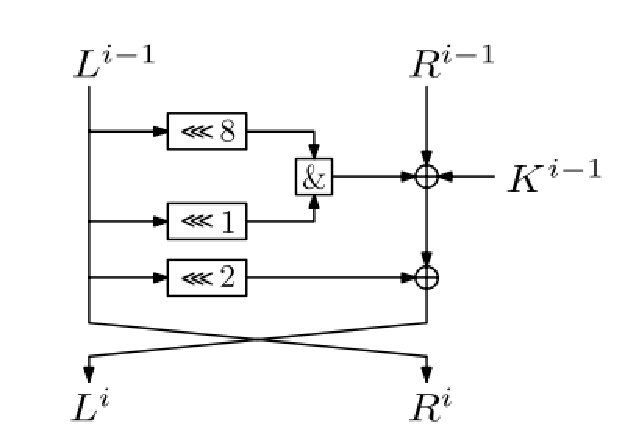
\includegraphics[width=120mm]{./pics/SIMONroundfn-eps-converted-to.pdf}
	\caption{The round function of SIMON}
	\label{fig:SIMONroundfn}
	\vspace{-0.1cm}
\end{figure}


The output of the last round is the ciphertext.

The key schedule of SIMON is based on an LSFR-like procedure, where the $nm$-bits of the key are used to generate the keys $K_0,K_1,...,K_{r-1}$ to be used in each round. There are three different key schedule procedures depending on the number of words that the secret key consists of ($m=2,3,4$).

At the beginning, the first $m$ words $K^0,K^1,...,K^{m-1}$ are initialized with the secret key, while the remaining are generated by the LSFR-like construction. For the variant of our interest, where $m=4$, the remaining keys are generated in the following way:

\begin{equation}
Y=K^{i+1}\oplus (K^{i+3}>>>3)
\end{equation}

\begin{equation}
K^{i+4}=K^i\oplus Y \oplus (Y>>>1)\oplus c\oplus (z_j)_i
\end{equation}

The constant $c=0xff...fc$ is used for preventing slide attacks and attacks exploiting rotational symmetries \cite{NSAciphers}. In addition, the generated subkeys are xored with a bit $(z_j)_i$, that denotes the $i$-th bit from the one of the five constant sequences $z_0,...,z_4$. These sequences are defined in \cite{NSAciphers} and for our variant we use $z_3$. In \cite{simonref} there is a basic reference implementation of SIMON and SPECK ciphers and a basic generator of equations that are used in algebraic attacks.

The Feistel network, the construction of the round function and the key generation of SIMON, enables bit-serial hardware architectures which can significantly reduce the cost of implementation \cite{simoneff}. Additionally, encryption and decryption can be done using the
same hardware.
\section{Algebraic Cryptanalysis of SIMON}

We evaluated the security of SIMON against algebraic attacks under the following
three settings (cf. Fig. \ref{ThreeScenarios}), where S=Similar and R=Random
as explained in the introduction.

\begin{itemize}
	\item \textbf{Setting 1:}(RP/RC) Random P-C pairs are available
	\item \textbf{Setting 2:}(SP/RC) Random P-C pairs are available with plaintexts of low Hamming distance
	\item \textbf{Setting 3:}(SP/SC) Random P-C pairs which satisfy a truncated differential property in the input and output of the reduced-version of the cipher we study. More random P-C pairs are generated and used.
	% \item \textbf{Setting 3':}(SP/SC)' Random P-C pairs which satisfy a truncated differential property in the input and output of the reduced-version of the cipher we study. Then we generate more such pairs by using pairs with similar plaintexts (low Hamming Distance)
	%    such that ciphertext pairs lie in the truncated differential mask.
\end{itemize}

\begin{figure}[!h]
	\vspace{-0.2cm}
	\centering
	%{\epsfig{file = three_scenarios.eps, width = 7.5cm}}
	\includegraphics*[width=60mm]{./pics/three_scenarios2.jpg}
	\caption{Our three attack scenarios}
	\label{ThreeScenarios}
	\vspace{-0.1cm}
\end{figure}



%\begin{figure}[h!]
%    \centering
%    \includegraphics{three_scenarios.eps}
%    \caption[width=0.2]{Our three attack scenarios}
%    \label{setting}
%\end{figure}

Setting 1 is the simplest setting of understanding how many rounds of SIMON
can be broken by simple guess-then-determine techniques, assuming availability of
a few P-C pairs. This setting help us to understand the maximum number of rounds we
can break by guessing as few as possible key bits and using as few as possible P-C
pairs. It a non-trivial step in order to set the benchmark for attacking more number of rounds.


Setting 2 is a form of known-plaintext attack. Setting 2 requires the existence of P-C pairs with plaintexts
of low Hamming distance (or similar plaintexts)
such that many variables are eliminated in the first few rounds due to weak
diffusion. By eliminating some variables from the initial equations we expect that
the system will be solved faster using any solving technique. This is a form of
chosen plaintext attack.

Lastly, Setting 3 assume the existence of P-C pairs

\begin{center}
	$\{(P_1,C_1),(P_2,C_2),...,(P_n,C_n)\}$
\end{center}

such that
$P_i\oplus P_j \in \Delta P$ and $C_i\oplus C_j \in \Delta C$, for
all $1\leq i,j \leq n$ and some truncated differential masks $\Delta P,\Delta C$
of low Hamming weight which holds with comparatively high probability.
In our attacks we always use 2 pairs which satisfy a given truncated
differential property and then more P-C pairs are generated by using the
first 2 plaintexts and computing the encryptions of new plaintexts which have small Hamming distance from the
first ones. 

The difference
from Setting 2 is that in this case we also eliminate variables
from the last rounds of the cipher, expecting that the system is even more easier to solve. In this
attack, we need assume that the entire codebook is available and thus the
data complexity is $2^{64}$.

In all of our attacks we start with an 8-round truncated differential property $\Delta=[00000222 00000080]$
with 4 active bits found by our discovery method which is the following

\begin{equation}
Prob(\Delta\rightarrow \Delta)\simeq2^{-20.51}
\end{equation}

The mask $[00000222 00000080]$ denotes the set of $2^4-1$ possible differences,
excluding the zero difference.
Our detailed results and discussion will be presented in the following section.

\section{Algebraic Attacks experiments and results}
We run experiments using SAT solvers and ElimLin Algorithm on a machine with the
following characteristics

\begin{itemize}
	\item CPU: Intel i7-3520m 2.9GHz
	\item RAM: 4G
	\item OS: 64-bit Windows 8
\end{itemize}

Our implementation of Simon can be found at \cite{simonref} which also include an equation generator which generate an algebraic equitation system for n round Simon encryption. Once the equation is generated, we use Nicolas Courtois' software \cite{EquationSolving} to either solve the system by ELimlin or convert to CNF file and then solved by a SAT solver. For reader to check and verify our results, here are the command line we used to get our experiments results:

\begin{itemize}
	\item ELimlin: xl0.exe /deg2 filePath
	\item SAT Solver: xl0.exe /deg2 /sat /bard /timeout600 /cryptominisat64296 filePath
\end{itemize}

\subsection{Experiments with 2 P/C pairs}
The initial benchmark experiments was done with only 2 P/C pairs and solved by SAT solver using 8 round Truncated differential mask $[00000222 00000080]$ $\Rightarrow$ $[00000222 00000080]$. Table \ref{tab:example1} presents our 2 P/C pairs experiment results. The average time (in seconds) taken $T_{average}$
to solve the underlying problem
by a SAT solver is presented, while the time complexity $C_T$
(in terms of SIMON encryptions) is
computed by the following formulae,

\begin{equation}
C_T=2^{k}\times2^{log_2(T_{average}*N_{8REnc})},
\end{equation}

where $k$ is the number of bits we guess initially, $N_{nREnc}$ is the number of n round Simon encryptions the experiment PC can run in 1 seconds.

\begin{table}[!hh]
	\caption{Best results obtained by a SAT solver}\label{tab:example1} \centering
	\begin{tabular}{|c|c|c|c|c|c|}
		\hline
		$\#$(Rounds) & $k$ & $\#$(P-C) & $T_{average}$(s) & $C_T$ & Setting \\
		\hline
		8 & 84 & 2 & 63.76   & $2^{110.08}$ & RP/RC \\
		8 & 80 & 2 & 87.38   & $2^{106.53}$ & RP/RC \\
		\hline
		8 & 75 & 2 & 156.60  & $2^{102.37}$ & SP/RC \\
		\hline
		8 & 75 & 2 & 515.60  & $2^{104.09}$ & SP/SC \\
		\hline
	\end{tabular}
\end{table}

We start from setting 1 using random Plaintext and random Ciphertext pair (RP/RC), until we can not solve the equations using SAT solver. We successfully break 8 rounds Simon with guessing some key bits. The best result for 8 rounds is fixing 80 key bits with complexity of $2^{106.53}$. Fixing less than 80 key bits will not be solved by SAT solver within 600 seconds. Then we try Setting 2 and Setting 3 to compare the results. Setting 2 using selected Plaintext and Random Ciphertext (SP/RC) and setting 3 using selected Plaintext and selected ciphertext (RP/RC) is better than RP/RC. However, the results in table \ref{tab:example1} show that SP/SC is not perform any better than SP/RC. Both SP/RC and SP/SC are not improving RP/RC a lot. 

The experiment results show that for setting 2 and setting 3, using only 2 P/C pairs can not provide enough information (additional linear equations) to perform a better attack than RP/RC. In the next subsection we try to increase the number of P/C pairs and compare the results using different settings.

\subsection{Experiments with more P/C pairs}
We start to using more P/C pairs for 8 rounds Simon and we show our results in talbe \ref{tab:8RmorePC}. Here we start to record some features of the converted CNF files. In table \ref{tab:8RmorePC} and other SAT solver results table, $n,s,h$ stand for number of variables, average sparsity (the average number of literals in each clause) and hardness respectively and $m$ is the number of clauses in the converted CNF file.
We define hardness as a number $h$ such that $h^n$ is the running time, where $n$ is the number of variables.
It is known that $h\leq 1.47$ for 4-SAT problems (cf. Table 1 in \cite{semaev})
% explain hardness

\begin{table}[!hh]
	\caption{Best results obtained by a SAT solver}\label{tab:8RmorePC} \centering
	\begin{tabular}{|c|c|c|c|c|c|c|c|c|c|}
		\hline
		$\#$(Rounds) & $k$ & $\#$(P-C) & $T_{average}$(s) & $C_T$ & Setting & $n$ & $x=\frac{m}{n}$ & $s$ & $h$ \\
		\hline
		8 & 45 & 6 & 207.31   & $2^{27.78}$ & RP/RC & 8576	& 6.5118	& 4.2761	& 1.0032 \\
		\hline
		8 & 0  & 6 & 12.21   & $2^{23.76}$ & SP/RC  & 8576	& 6.5065	& 4.2787	& 1.0029  \\
		\hline
		8 & 0  & 6 & 11.84   & $2^{23.57}$ & SP/SC  & 8576	& 6.5513	& 4.2631	& 1.0028 \\
		\hline
	\end{tabular}
\end{table}

From Table \ref{tab:8RmorePC} we can see that when using more P/C pairs, all the three settings get better results than using 2 P/C pairs in Table \ref{tab:example1}. The improvements for setting 2 and setting 3 are much more larger than setting 1. Setting 2 and setting 3 can break 8R Simon without guessing any key bits.

Then we start to extended the current 8 rounds attack to 9 and 10 rounds. We first extend our 8R truncated differential mask to 9 and 10 rounds as the following:
\begin{itemize}
	\item 9R: $[00000022 00000080]$ $\rightarrow$ $[00022e4c 00000222]$
	\item 10R: $[00000022 00000080]$ $\rightarrow$ $[002eff9a 00022e4c]$ 
\end{itemize}

We manage to break 9 rounds without guessing any key bits and break 10 rounds with some key bits guessing. Our best results are shown in table \ref{tab:10RmorePC}

\begin{table}[!hh]
	\caption{Best results obtained by a SAT solver}\label{tab:10RmorePC} \centering
	\begin{tabular}{|c|c|c|c|c|c|c|c|c|c|}
		\hline
		$\#$(Rounds) & $k$ & $\#$(P-C) & $T_{average}$(s) & $C_T$ & Setting & $n$ & $x=\frac{m}{n}$ & $s$ & $h$ \\
		\hline
		9 & 0 & 6 & 222.50   & $2^{27.9}$ & SP/RC & 9536	& 6.70	& 4.31	& 1.0029 \\
		9 & 0 & 7 & 94.7   & $2^{26.6}$ & SP/RC & 11104	& 6.70	& 4.31	& 1.0024 \\
		10 & 90 & 8 & 346.0   & $2^{118.5}$ & SP/RC & 13952	& 6.90	& 4.32	& 1.0020 \\
		\hline
		9 & 0  & 6 & 24.24   & $2^{24.7}$ & SP/SC  & 9536	& 6.69	& 4.31	& 1.0026  \\
		9 & 0  & 7 & 18.56   & $2^{24.3}$ & SP/SC  & 11104	& 6.70	& 4.31	& 1.0022  \\
		10 & 70  & 10 & 417.73   & $2^{98.79}$ & SP/SC  & 17408	& 6.88	& 4.31	& 1.0022  \\
		\hline
	\end{tabular}
\end{table}

Moreover, assuming Setting 3 we can break 10 rounds by
guessing 70 bits of the key initially with time complexity $2^{98.79}$ encryptions.
Note that in SP/SC setting we always generate two P-C pairs which satisfy the truncated differential property and the rest pairs are generated at random.

The other two settings have failed to produce good results for 10 rounds in reasonable time
and this reflects the power of using pairs which follow strong truncated differential properties. We conjecture that for a cipher of low MC, there exists a certain amount of pairs which depends on the MC which can be used to break any round.

\subsection{Algebraic Attacks Using ElimLin Algorithm}

Table \ref{tab:SimonElimlin} presents the results using the ElimLin algorithm for solving the
underlying system of equations.


\begin{table}[!h]
\caption{Best results obtained by a ElimLin Algorithm}\label{tab:SimonElimlin} \centering
\begin{tabular}{|c|c|c|c|c|c|}
  \hline
  $\#$(Rounds) & $k$ & $\#$(P-C) & $T_{average}$(s) & $C_T$ & Setting \\
  \hline
  8 & 0 & 6 & 824.4 & $2^{29.8}$ & SP/RC \\
 \hline
 8 & 0 & 6 & 583.2 & $2^{29.3}$ & SP/SC \\
  \hline
\end{tabular}
\end{table}

ElimLin exploits the existence of linear equations in order to solve the system. We have been able to break up to 8 rounds in Setting 3 without guessing any key bits
initially. Setting 1 fails while Setting 2 is much weaker than Setting 3. The best
attack we have obtained is of time complexity $2^{29.3}$ encryptions against 8 rounds of SIMON and requires pairs which satisfy
the truncated differential property presented in the previous section extended for 8 rounds.

Adding pairs which follow a strong truncated differential property is equivalent to adding linear equations in the system and this
is exploited by the ElimLin algorithm. An immediate improvement is to use additional intermediate truncated differences.
This will eliminate also variables in intermediate rounds and introduce more linear
equations in the intermediate rounds. We conjecture that ElimLin is more powerful
in case where a strong characteristic is found by our discovery method (intermediate difference states).

%secrypt2016 
%TODO

\section{ElimLin On Lightweight Ciphers}
Our initial algebraic cryptanalysis work on Simon was published in 2014. In 2015,   Raddum \cite{RaddumSimon} published another algebraic cryptanalysis on more version of Simon and have break many rounds using Elimlin with more P/C pairs. 

 
However, a major difficulty with ElimLin is that so far it has been successful only for relatively simple lightweight ciphers.
For more complex ciphers
%%% full version maybe %%%
%%it is not clear if the attack makes big progress.
it seems to do things which are relatively trivial,
%However until now this has not been formalized.
%We do not know what trivial means.
%for example
e.g. equations generated do not penetrate deeply inside the cipher, or very slowly,
cf. %for example
slide 153 in \cite{SlidesAlgAllteach}.
% we observe that as the number
%of new linear equations grows,
%these equations penetrate more and more deeply inside the cipher for $2,3,5,\ldots$ rounds.

My work aim to make some definite progress in the direction of distinguishing between trivial and non-trivial behavior for ElimLin. This is not only about penetrating deeper inside the cipher. Previous experience shows that ElimLin only starts to work at a certain threshold. Before this threshold, again nothing non-trivial can be observed even though slow penetration occurs. This is not really apparent in any of the current works or is lost in vast quantities of data generated in computer simulations. 
%In this paper we are going to be the first to define what non-trivial means.
We define a new criterion which shows that it is possible to see that there exist two very different and easily distinguishable patterns in ElimLin. Either the attack follows one pattern, and does nothing trivial, or it follows another pattern and it is very clearly doing well.

\subsection{Phase transitions}

It is known that many NP-hard problems are subject to ``phase transition'', with certain parameters that problem is hard, and then will rather abruptly transition from ``hard'' to ``easy to solve''. This is what we observe with ElimLin. % here. 
Let $K$ be the number of Plaintext/Ciphertext (P/C) pairs used in an ElimLin attack. We are going to discover that at a certain threshold the number of new linear and linearly independent equations
generated at various stages of the attack can follow one curve,
and then switch to another curve with a different asymptotic growth rate.



%\begin{conj}
{\bf Conjecture \ref{ElimLinQuadConj}}
\label{ElimLinQuadConj}
Consider a system of multivariate equations derived from a block cipher written following
one of the two basic strategies described in \cite{desalg,SlidesAlgAllteach}.
Consider a simple known plaintext attack with $K$ Plaintext/ciphertext (P/C) pairs.
Consider a case such that the cipher is eventually broken by ElimLin, cf. \cite{FastAlg,FastAlg2,ToyRijSer,AlgteachElimLinLab,RaddumSimon}.
The number of new and linearly independent linear equations generated
by ElimLin algorithm goes through several distinct stages St0-St3:

\begin{enumerate}
	\item[St0]
	Initially it grows linearly with $K$,
	and for certain individual stages of the attack is
	simply equal to 0 and does NOT grow,
	cf. our later $r_i$ notation in Section \ref{ElimLinNotation}.
	\item[St1]
	Then it switches to another curve where
	it grows faster than linearly in $K$.
	%cf Sec. \ref{SuperLinearGrowth}
	\item[St2]
	This until it reaches a saturation stage where the
	cipher is completely broken by ElimLin.
	Here we have a very rapid phase transition cf. Section ref{BigPictureUpAndDown}
	where the number of equations $r_i$ generated at one stage re-becomes 0
	simply because an earlier stage of the attack reaches a certain threshold where combinatorial explosion
	in additional equations generated
	makes it complete the whole attack and not requite the next stage to be executed].
\end{enumerate}

\noindent
%Again let $K$ be the number of P/C pairs in an ElimLin attack.
One (old) example from 2007 which shows that the number of equations grows faster than linear
as a function of the data complexity $K$ in ElimLin
can be found at slide 153 in \cite{SlidesAlgAllteach}
and which originally comes from \cite{ToyRijSer}. 
%ToySerpent but not ToyRijndael [or more data are needed]
%%% full version maybe %%%
%This paper
%%is dedicated to see if this conjecture is verified in the real life
%and how exactly we can approximate different stages of the attack by precise closed formulas
%which allow to predict the outcomes of the attack as exactly as possible.


%\newpage

%\section{\uppercase{Our Experimental Setup and Notation}}

\section{Experimental Setup and Notation}
\label{ElimLinSetup}
\label{ElimLinNotation}

More examples can be easily obtained using a basic software setup which we use at UCL to run
a hands-on student lab session on algebraic cryptanalysis of block ciphers \cite{AlgteachElimLinLab},
which is part of GA18 course on cryptanalysis taught at UCL.
One example could be easily obtained for the CTC2 cipher, cf. \cite{FastAlg,FastAlg2,AlgteachElimLinLab}.
A more ``modern'' example can be generated by using the equations generator for Simon block cipher
developed by Guangyan Song and UCL student Ilyas Azeem in 2015-6,
%TODO developed in cryptyanalysis of simon
the complete source code of which is
available at github, cf. \cite{AlgteachElimLinLab,CourtoisSoftware}.
The ElimLin is executed using one of our implementations of
ElimLin \cite{AlgteachElimLinLab,CourtoisSoftware} which has the nice particularity to display on screen the number of linear equations generated at each stage/iteration of the algorithm.

We recall the two main and only steps of ElimLin:

\begin{enumerate}
	\item[1] Find $r_i$ linear equations in the linear span, $i=0,1,2,3,\ldots$.
	\item[2a] If $r_i>0$ eliminate some $r_i$ variables,
	increment $i$ and try again Step 1.
	\item[2b] Algorithm terminates when $r_i=0$ for some $i$.
\end{enumerate}

In addition and by convention we are going to define a step $i=0$ which is different than
above, but the same which is implemented in a common implementation of ElimLin \cite{CourtoisSoftware}.
We will assume that $r_0$ will be the number of linear equations which already appear in the equations,
without executing any linear algebra. This is a convention which allows researchers to distinguish
more easily between a ``misleading'' starting number of variables (which is sometimes artificially inflated due to
methods used for equation generation and formal coding)
and the ``real'' or intrinsic number of variables which is there prior to execution or ElimLin.

%\begin{defi}[ElimLin progress indicators]\\
{\bf Definition \ref{ElimLinProgressParams}[ElimLin progress indicators]}\\
\label{ElimLinProgressParams}
Let $V_{start}$ or simply $V$ if there is no confusion
be the initial number of variables.
We define by $r_i$ the number of
linear/affine equations over GF(2)
generated at each stage of the algorithm
where by convention $r_0$ is the number of
linear/affine equations over GF(2) already present.
We define

\begin{equation}
V^i_{broken}=\sum_{j=0}^{i} r_j ~~~~~~~~V_{broken}=\sum_{i=0}^{\infty} r_i
\end{equation}

where by convention $r_i=0$ if algorithm has reached
$V^i_{broken}=V$ at an earlier stage.
We define also

\begin{equation}
V^i_{broken}=V-\sum_{j=0}^{i} r_j
\end{equation}

and accordingly let
$
V_{unbroken}=V-\sum_{i=0}^{\infty} r_i.
$
Overall we will say that the algorithm terminates if
$V_{broken}=V$ and $V_{unbroken}=0$ and we deliberately ignore the fact that
some variables could be subject to a brute force step,
cf. FXL method in \cite{XL2}.
Overall our goal is to achieve for a certain $i$ that
\begin{equation}
\frac{V^i_{broken}}{V_{start}}=1
~~~~~~~~~~~\mbox{or}~~~~~~~~~~~~
\frac{V^i_{unbroken}}{V_{start}}=0
\end{equation}


%\end{defi}

\section{How to Predict the Success of ElimLin}

We start by a simple example which shows that accurate prediction is feasible.

\subsection{On Growth Rate in ElimLin}
\label{SuperLinearGrowth}

On the figure below we show the number of linear equations generated at stage 4 [counting from 0]
of the ElimLin algorithm for 8 rounds of Simon block cipher.
We should note that nothing remarkable happens at earlier stages 0,1,2,3,
the growth is linear and therefore very easy to predict.
We have then asked Microsoft Excel to produce a polynomial interpolation for this data series.

\begin{figure}[!h]
	\vspace{-0.2cm}
	\centering
	\includegraphics*[width=120mm]{./pics/image011.png}
		\caption{Number of linearly independent equations generated at stage 4
			of the ElimLin algorithm
			for 8 rounds of Simon 64/128 obtained with the exact software setup
			of \cite{AlgteachElimLinLab}.}
	\label{ElimLinQuadConjExampleSimon8}
	\vspace{-0.1cm}
\end{figure}

\subsection{Analysis of Our Prediction}

First property we need to note is that the polynomial prediction seems to be the right tool here.
This is justified by the fact that the normalized squared error value $R^2$ is very high and close
to the theoretical maximum of $1$, and also
that high degree coefficients are substantially smaller
(in absolute values) that lower degree polynomial coefficients.

%Our conclusion is as follows.
Secondly we observe that
%{\bf Conclusion.}
ElimLin eventually breaks the cipher here because
the number of newly generated linear equations grows
%{\bf asymptotically faster}
faster
than the number of variables which grows linearly with $K$.
Eventually we obtain a sufficient number of linear equations which makes ElimLin
compute all the variables and obtain the 128-bit secret key together with all the intermediate variables.
%
%%% full version maybe %%%
%{\bf Growth vs. Penetration.}
This was previously observed in other cases where ElimLin was applied
%and even barely starts to work... => explosion
cf. %for example slide 153 in
\cite{SlidesAlgAllteach,ToyRijSer,%FastAlg,
	FastAlg2,desalg} %,AlgteachElimLinLab}.
%%% full version maybe %%%
%In the table at slide 153 in \cite{SlidesAlgAllteach} we observe that as the number of new linear equations grows,
%these equations penetrate more and more deeply inside the cipher for $2,3,5,\ldots$ rounds.
%We expect the same to happen for other block ciphers when ElimLin was applied.

\subsection{Limitations vs. Improvements}

%{\bf Can This Fail.}
We do not know any %real
counter-example which would contradict our asymptotic super-linear growth rule.
For 8 rounds of Simon cipher we observed that the growth remains strictly linear for
equations computed at stage 3, however some equations are only computed at stage 4
and this occurs quite early starting from $K=1$.
However Simon is a particularly simple cipher. For more complex ciphers,
the ElimLin algorithm could have serious problems to enter this behavior
or start working and exhibit any sort of non-trivial behavior.
However when ElimLin starts to work for some cipher and produces new equations
which depend on the plaintext or ciphertext data in a non-trivial way,
steady progress is observed.
%it seems that nothing can stop it.
Except maybe if there isn't enough data available.
A certain type of counter-example could occur for some ciphers
with small blocks which
would maybe not be able to allow $K$ to be large enough for ElimLin to terminate.

{\bf Improvements.}
We stress that this powerful phenomenon of combinatorial explosion which eventually leads
to ElimLin breaking the cipher
occurs already for a basic straightforward application of ElimLin in a
known-plaintext attack (KPA) scenario.
Several methods to make ElimLin work better by using
well-chosen P/C pairs.
One method which has been used ever since ElimLin was invented \cite{FastAlg,FastAlg2,desalg}
is to exploit a CPA (chosen-plaintext attacks) with plaintext which differ by extremely few bits, for example in a counter mode.
More recently new methods have been proposed
%in the literature
which allow to generate additional linear equations
not automatically discovered by ElimLin
\cite{ACTruncSimon} and \cite{ElimLinUniversalEqs}.
%2 very different mechanisms...

In this paper we again focus on very simple variants of ElimLin in order to show that
{\bf high accuracy} predictions (e.g. with $R^2\approx 1$) are possible to achieve.
This success should encourage and set up standards for further research
on more realistic and more powerful but also more complex applications of ElimLin, cf.
\cite{ACTruncSimon,ElimLinUniversalEqs,RaddumSimon}.

%\newpage

\section{The Big Picture - Long Term Predictions}
\label{BigPictureUpAndDown}

As already explained in
Conjecture \ref{ElimLinQuadConj}
page
\pageref{ElimLinQuadConj},
we expect that there are at least 3 distinct stages in ElimLin algorithm.
With these notations until now we have been only looking at stage St1 of the attack.
In this section we look at the big picture and the main phase transition
ST1-2 which is the most fundamental one because we have really here a
transition from ``hard'' to ``easy'' and some sort of
combinatorial explosion in the number of generated equations at one stage
which for even higher $K$ makes this stage $i$ of the attack unnecessary
because the  attack will terminate at an earlier stage $i-1$.
%%% full version maybe %%%
%and a similar rapid growth will be observed for $r_{i-1}$ value.
This is best seen by looking at how the value of $V_{unbroken}$ evolves with growing $K$.

\begin{figure}[h!]
	\vspace{-0.2cm}
	\centering
	\includegraphics*[width=120mm]{./pics/pol4_U.png}
	 \caption{Number of variables when ElimLin terminates  $V_{unbroken}$
	 	for 8 rounds of Simon 64/128 obtained with the exact software setup
	 	of \cite{AlgteachElimLinLab}.}
	 \label{ElimLinUnrokenCurveUpDownSimon8}
	\vspace{-0.1cm}
\end{figure}

This curve seems a lot harder to predict than until now.
For example we have obtained the following polynomial predictor

\begin{multline}
V_{unbroken}(K)=\\
-\frac{1.35}{10^4}
K^4
+
\frac{2.07}{10^2}
K^3
-
1.12\cdot K^2+
22.4\cdot K + 308.25
\end{multline}

for which we have $R^2=0.9863$.
Substantially better accuracy can be achieved by focusing on another quantity
and looking at a wider range or prediction methods.
We have tried many different predictors obtained with Microsoft Excel and WolframAlpha cloud
online service \url{www.wolframcloud.com} which offers higher precision and more advanced functionalities.
In general focusing on the ratio $V_{unbroken}/V_{start}$ gives substantially better results,
as $V_{start}$ grows linearly with $K$ and our primary interest in this paper is a deviation
from that linear growth which is the default (trivial) behavior. The curves become then more regular and
more intelligible, cf. later Figure \ref{CTC2StrongerThanSimon7RCurve}.
For example we obtained $R^2=0.9941$ with

\begin{equation}
\frac{V_{unbroken}(K)}{V_{start}}=
1.07 \cdot x^{-0.485} -0.127
\end{equation}


Then we obtained $R^2=0.9989$ with a polynomial of degree 6:
%(best precision available in Excel):

\begin{multline}
\frac{V_{unbroken}(K)}{V_{start}}=
-
\frac{2}{10^{10}}K^6
-
\frac{5}{10^8}K^5
+
\frac{5}{10^6}K^4\\
-
\frac{3}{10^4}K^3
+
\frac{7.5}{10^3}K^2
-
0.112 K
+0.8083
\end{multline}


%y = 2E-10x6 - 5E-08x5 + 5E-06x4 - 0.0003x3 + 0.0075x2 - 0.112x + 0.8083

Finally we have obtained an even better result $R^2=0.9998$ with

\begin{multline}
\frac{V_{unbroken}(K)}{V_{start}}=
-\frac{9.57}{10^3}(\ln K)^4
+\frac{1.00}{10}(\ln K)^3\\
-\frac{3.19}{10}(\ln K)^2
-\frac{1.35}{10}\ln K
+0.65.
\end{multline}


{\bf Goals.}
%{\bf Research Objectives.}
Overall %we propose that
in security of block ciphers
the main goal for further development of prediction techniques
will be first
to predict the moment when the curve on
Figure \ref{ElimLinUnrokenCurveUpDownSimon8} starts falling.
This is the main phase transition from ``hard'' to ``easy'' in any ElimLin attack.

\subsection{Are Reliable Extrapolations Possible?}
\label{BigPictureUpAndDown2}

So far we have only worked with data from simulations and all our predictions are highly accurate
just because we had quite a few data points and have deployed sufficient effort to compute predictors with standard techniques.
The fact that {\bf several methods} give remarkably good results
should however be a warning sign.
This together with insufficient amount of data will be a major difficulty %primary topic of interest
when researchers in the future are going to
try to build predictive models to extrapolate and compute the complexity of simulations
which they have not done.
In an extrapolation scenario it is easy to see that %what will happen is that
even though different methods used will give excessively good results on the actual data in a certain interval,
they could diverge and could fail to predict the curve on a larger interval.
Even in this case these predictions can be used to determine
the possible or plausible range of results which one can expect to achieve.
%This makes our predictions more hazardous. % and less clear

A real solution for this difficulty would be to have an
``\`{a} priori'' idea
about the nature of the curve and its growth.
We had that in Section \ref{SuperLinearGrowth} and the polynomial approximation
has larger degree coefficients which have decreased rapidly
confirming our ``\`{a} priori'' idea on super-linear growth approximated by a polynomial.
%%WE DO!!!! ...?We do not have this ``\`{a} priori'' theoretical or heuristic prediction of any sort.
Here for predicting $V_{unbroken}(K)$ which is essentially proportionnal ot sum of the $r_i$
we also expect a polynomial prediction and we obtained $R^2=0.9989$.
This is also a somewhat consistent predictor with
rapidly decreasing coefficients of higher degree.
If so, shouldn't we use a lower degree predictor?
% lowering the degree
%%%VERY BAD To cut it
%which could be just simplified to
%$\frac{V_{unbroken}(K)}{V_{start}}=0.09K+0.76$.
%How accurate is this simplification on our complete set of data ??_ BAD!!! see new graph added tab K-US8 in SimonResults2.xlsx...

%\newpage
\subsection{Are Low Degree Polynomial Extrapolations Possible?}
\label{BigPictureUpAndDownLowDegreeFails}

%{\bf Important Remark.}
If we look at our later Figure \ref{CTC2StrongerThanSimon7RCurve} or again how quickly
lower degree coefficients decrease in predictors above,
we could be tempted to use a linear or low degree predictor.
%knowledge
Our experience shows that cutting small higher degree terms in these predictors is disastrous
and does not lead to quality predictions,
not even on smaller intervals.
For example we can cut the beginning of current series
and restrict to polynomials of degree 2 for $\frac{V_{unbroken}(K)}{V_{start}}$
and we obtain a predictor of
$
\frac{V_{unbroken}(K)}{V_{start}}\approx
\frac{6}{10^5}K^2
-\frac{7.7}{10^3}K
+0.26
$
which is neither very consistent with more accurate predictors computed above
nor with the data trend at most places.

\begin{figure}[h!]
	\vspace{-0.2cm}
	\centering
	\includegraphics*[width=120mm]{./pics/KUS8_deg6.jpg}
	\includegraphics*[width=120mm]{./pics/KUS8_deg2.jpg}
    \caption{Good vs. bad predictors:
	decreasing the degree of a polynomial prediction
	for the same Simon 64/128 8 rounds. %\cite{AlgteachElimLinLab}.
}
    \label{ElimLinUnrokenCurveUpDownSimon8BadPRedictorCurDeg2}
	\vspace{-0.1cm}
\end{figure}

The latter graph is definitely not a predictor we would recommend!
%Further research on this topic is needed.

%\newpage
\section{On Comparative Strength of Ciphers}
\label{SimonWeakerThanCTC2}

Another major application of ElimLin techniques and possible extrapolations
is to make comparison between different ciphers.
For example current research indicates that Simon is broken for up to 16 rounds
\cite{RaddumSimon} and CTC2 for up to 7 rounds, both using ElimLin algorithm.
Is it possible to claim that one round of Simon is substantially weaker than one round of CT2?
We would agree with this claim. On the figure below we show how the quantity
$\frac{V_{unbroken}(K)}{V_{start}}$ decreases for 7 rounds for each cipher.
We conclude that both ciphers are broken for some $K$ value but with ElimLin we still have a long way to go before the attack terminates resulting in much higher data complexity and running times.
%
This shows that there exist ciphers fundamentally weaker than CTC2 even though CTC2 was designed
to be quite vulnerable to algebraic attacks \cite{FastAlg,FastAlg2}.
%%% full version maybe %%%
%and %even though
%we looked at a weak variant of CTC2.

%\newpage
\begin{figure}[h!]
	\vspace{-0.2cm}
	\centering
	\includegraphics*[width=120mm]{./pics/SimonvsCTC2_7.jpg}
	\caption{The value of $\frac{V_{unbroken}(K)}{V_{start}}$ for 7 rounds of
		Simon 64/128 (blue) compared to toy cipher CTC2 with 7 rounds
		and 8 S-boxes per round and 10/24 key bits known (red).}
	\label{CTC2StrongerThanSimon7RCurve}
	\vspace{-0.1cm}
\end{figure}

This per-round weakness of Simon is expected to be compensated by a larger number of rounds.
%Now the cryptographic history shows that ciphers which have been designed to be secure
%for a larger number of rounds \cite{gostac}


%%% full version maybe %%%
%Overall we need to realize that that ElimLin can break way more than 16 rounds of Simon as reported in
%\cite{RaddumSimon} and extrapolations are needed and can be obtained with the methods of this paper.
%In particular Figure \ref{CTC2StrongerThanSimon7RCurve} seems very promising as it seems to
%be very regular and exempt from sudden changes of direction which we have observed on
%Figure \ref{ElimLinUnrokenCurveUpDownSimon8}.
%However truly accurate prediction
%%is not going to be easy.
%can NOT be achieved by extending this curve and assuming that it is linear,
%this gives very bad results,
%see Section \ref{BigPictureUpAndDownLowDegreeFails}.
%We expect that much better results will obtained by polynomial interpolation
%as shown in Section \ref{BigPictureUpAndDown}.




